%
% Honours Report Template
% updated May 2013
%
\documentclass[a4,12pt]{article}
\makeatletter
\renewcommand\paragraph{\@startsection{paragraph}{4}{\z@}%
            {-2.5ex\@plus -1ex \@minus -.25ex}%
                        {1.25ex \@plus .25ex}%
                                    {\normalfont\normalsize\bfseries}}
                                    \makeatother
                                    \setcounter{secnumdepth}{4} % how many sectioning levels to assign numbers to
                                    \setcounter{tocdepth}{4}    % how many sectioning levels to show in ToC
%
\usepackage{epsfig}
\usepackage{latexsym}
\usepackage{graphicx}
\usepackage{./natbib/natbib}
% It also sets the bibliographystyle to plainnat; for more information on
% natbib citation styles, see the natbib documentation, a copy of which
% is archived at http://www.jmlr.org/format/natbib.pdf
\usepackage{setspace}
\usepackage{amsmath}
\usepackage{amssymb}
\usepackage{amsfonts}
\usepackage{color}

%\graphicspath{{./figures/}
%Formatting-------------------------------------------------------------------
%\renewcommand{\refname}{\textbf{Literature}}
%
\renewcommand{\contentsname}{\small\textbf{{\center Table of Contents}}}
%
\setlength{\textheight}{8.8in}
%
\setlength{\topmargin}{-1.5cm}
%
\doublespacing
%\setlength{\textwidth}{17cm}
%
%\setlength{\oddsidemargin}{-0.1714in}
%
% Boxit -----------------------------------------------------------
\setlength{\fboxrule}{0.2mm} \setlength{\fboxsep}{4mm}
%
\newsavebox{\savepar}
\newenvironment{boxit}{\begin{lrbox}{\savepar}
        \begin{minipage}[b]{4.6in}}
        {\end{minipage}\end{lrbox}\fbox{\usebox{\savepar}}}
        
        
        
        
 \hyphenation{op-tical net-works Mathe-ma-tical street-scape street-scapes aes-the-tics aes-the-tic com-pu-ting geo-metric Geo-me-tric geo-metry boun-da-ries de-ve-lop-ment know-ledge mani-fold mani-folds high-di-men-sio-nal}
%
%
%
% Document-----------------------------------------------------------------------
%
\begin{document}
%
\title{\bf Technology \& User Engagement}
%
\author{Ross Bille\\
School of Electrical Engineering \& Computer Science\\
The University of Newcastle\\ Callaghan NSW 2308, Australia\\
Email: \texttt{c3127333@uon.edu.au} } 
\maketitle


\newpage
\begin{abstract}%
\noindent The abstract summarises the content of the paper or report and should have 70-200 words (depending on the publisher or other requirements); It
should state briefly what the paper is about (maybe also what
methods were used), what its (new) results are, why it is
important or significant. It can also be useful to state (or
indicate implicitly) who is the addressed readership and whether
its a review article, a short paper, a pilot study, an
extension of previous work or a thesis. Try to avoid special symbols, abbreviations, and citations.
\end{abstract}

\pagebreak

\tableofcontents

\pagebreak

\section{Introduction}
test~\citep{test}
There are different ways to write an introduction. Typically it
contains background information and a review of literature which
indicates how the study fits into the context of other previous
work. This way the introduction can  address the significance and importance of the study. Major related publications in big journals should be cited
as well as closely related other articles. The literature review typically uses newer papers when it tries to address the state-of-the-art of a technique or recent developments. However, when first mentioning a method name the historically first source that introduced that concept should be cited. There are different citation styles and here is an example~\citep{QuinlanChalupMiddletonACRA2003}. The introduction
typically motivates the general hypotheses, aims and research questions
of a paper, report or thesis.  

%Confidence in technology
%    how to get the genreal community interested in using current technology in order to drive research

\begin{center}
\begin{boxit}
\textbf{How do we get users more involved in the systems we create?}
\end{boxit}
\end{center}

Questions raised in the introduction can later be answered in the final discussion.

The introduction often ends with a brief overview of the structure or organisation of
the paper, report or thesis.

%
\section{Background}
Why we need user engagement
\subsection{The Skinner Box}
The Skinner Box is a technique named by B.F. Skinner describing a small cage which houses a small animal, a lever and a way of delivering rewards to the animal (Slater, 2005). The idea was to train the animal to continuously hit the lever. The animal gets rewarded at random intervals for lever pressing, with the possibility of punishment if the lever is not pressed (usually by electric shock). This technique has been around since the 1930’s and has been implemented in video games since their inception.
\\
Game designers have expanded the Skinner Box concept and made it feel like second nature to players. They have done this by offering virtual rewards to players who achieve pre- defined goals (this is obvious in any games that have levels and/or virtual currency) and recently by punishing players for not playing regularly (usually by devaluing the players hard earned virtual currency or by making in-game possessions deteriorate).
\\
The Skinner Box concept is a great way to develop players’ obsession to a game while offering no real world reward, often leaving the player wondering why they wasted so much time on the game \citep{QuinlanChalupMiddletonACRA2003}
(“5 Creepy Ways Video Games Are Trying to Get You Addicted,” n.d.).
\subsection{Gamification}
Gamification is the process of integrating game dynamics and techniques into non-game processes. This is usually done to increase interaction, productivity or satisfaction.
\subsubsection{The history of Gamification}

\subsection{Virtual Reality}
\section{Elements in Game Design}

\subsection{Stories}
\subsection{Rewards}
\subsection{Usability}
\subsubsection{Effort Reduction}
\subsection{Competition}
\subsection{Environment}
%
\section{Existing Projects}
%
\subsection{Unit9}
Unit9 is a production company involved in some of the latest high-tech advertising, gaming, and interactive systems. Unit9's projects combine the latest mobile technology such as:
\begin{itemize}
    \item{Accelerometer}
    \item{GPS}
    \item{Web (HTML5 etc.)}
\end{itemize}
In order to create interactive:
\begin{itemize}
    \item{Advertisment}
    \item{Game}
    \item{Augmented Reality}
    \item{E-commerce}
\end{itemize}
systems.
Unit9 benefits greatly from the technique of gamification.
\subsection{City Evolutions}
``City Evolutions is an exciting collaboration between the City of Newcastle and the University of Newcastle. Ten sites within Watt Street will be lit up between sunset and 10pm, with digital projections on to selected walls and buildings for a year. The projections at each site will reflect and critique the fascinating history of Watt Street.'' (Tucker, 2013, p.4)
\\
The sites running on Watt Street offer differing levels of interactivity; from no interactivity (the user only views) to low levels of interactivity, i.e. the user can move an object left and right by moving in front of a camera or the user can press buttons on their android smart phone to select movies to be projected.
\subsection{Vivid}
\section{Proposal for the City Evolutions project}
\subsection{Hardware}
\subsubsection{Mobile}
\paragraph{NFC}
\paragraph{QR Codes}
\paragraph{Networking}
\subsection{Software}
\subsubsection{Gamification}
%outline the techniques in gamification and how they relate to the city evolutions (how ot be implemented)

\subsubsection{Closing the Loop}
\subsubsection{Social Media}
%http://www.go-gulf.com/blog/smartphone/
The City Evolutions team are already taking advantage of technologies such as NFC chips and QR codes. A suggestion would be to utilise them even more extensively. Some examples include:
\begin{itemize}
    \item{Develop a Login system and use NFC as a log in option}
    \item{Create leader boards where appropriate to encourage users to use the above mentioned Login system}
    \item{Make use of a digital checkin system so users can scan their smartphone
            \begin{itemize}
                \item{Rewards System (i.e. frequent visitor card)}
                \item{Popularity/rating register (i.e. to inform tourists of some of the popular destinations of visit in Newcastle)}
            \end{itemize}
        }
\end{itemize}
\section{Literature Review}
% compare + contrast different authors views 
% group authors who draw simmilar conclusions
% criticise aspects of methodology
% Note areas of authors disagreement
% Highlight exemplary studies
% Highlight gaps in previous research or questions left unanswered
% condlue by summarising what the literature says

\subsection{Work Place}
\subsection{Education}
\subsection{Community}

\subsection{Patterns}
% id patterns or trends in literature
\subsection{Relation}
% show how your study relates to previous studies
% show how your study relates to the literature in general
\subsection{Conclusions}
% http://www.canberra.edu.au/studyskills/writing/literature
%\subsection{CSSE Honours Thesis Specifications}\label{sec:thesis}
%For several years CSSE required the following specifications for an Honours report:
%\begin{itemize}
%\item Cover page, containing title, student name, submission date and supervisor name.
%\item Minimum of 50 pages, using 12 point font and double spacing (but at least 10,000 words).
%\item Minimum of 25 references.
%\end{itemize}
%\subsection{Assessment} \label{sec:assessment}
%Assessment of an Honours report would typically look points such as:
%\begin{itemize}
%\item Clear understanding of the topic of the work.
%\item Literature review (analysis, citations, organization, comprehensiveness).
%\item Clear problem definition and description.
%\item Methods applied to solve the problem (complexity, suitability).
%\item Comparison of alternative approaches, identification of the problems.
%\item Results/analysis/conclusion.
%\item Report presentation
%\end{itemize}
%
\section{Methods}
\subsection{Research}
\subsection{Observation}
Being a part of the City Evolutions team i have had access to a number of statistical data around the current level of interaction between the users and the various City Evolutions projects. Some of this data includes:
\begin{itemize}
    \item{Number of QR codes scanned (see table~\ref{table:qrcodes})}
    \item{Number of NFC chips scanned (see table ~\ref{table:nfcchips})}
    \item{Number of interactions with various applications (see table~\ref{table:cityEvolutionsProjects} and figure~\ref{fig:nn1})}
\end{itemize}
Figure~\ref{fig:nn1} shows the level of interaction over time of users with the City Evolutions Threkeld system.
% TODO: add a graphical representation of interaction over time of Threkeld
\begin{figure}[htbp]
\begin{center}
    \leavevmode
    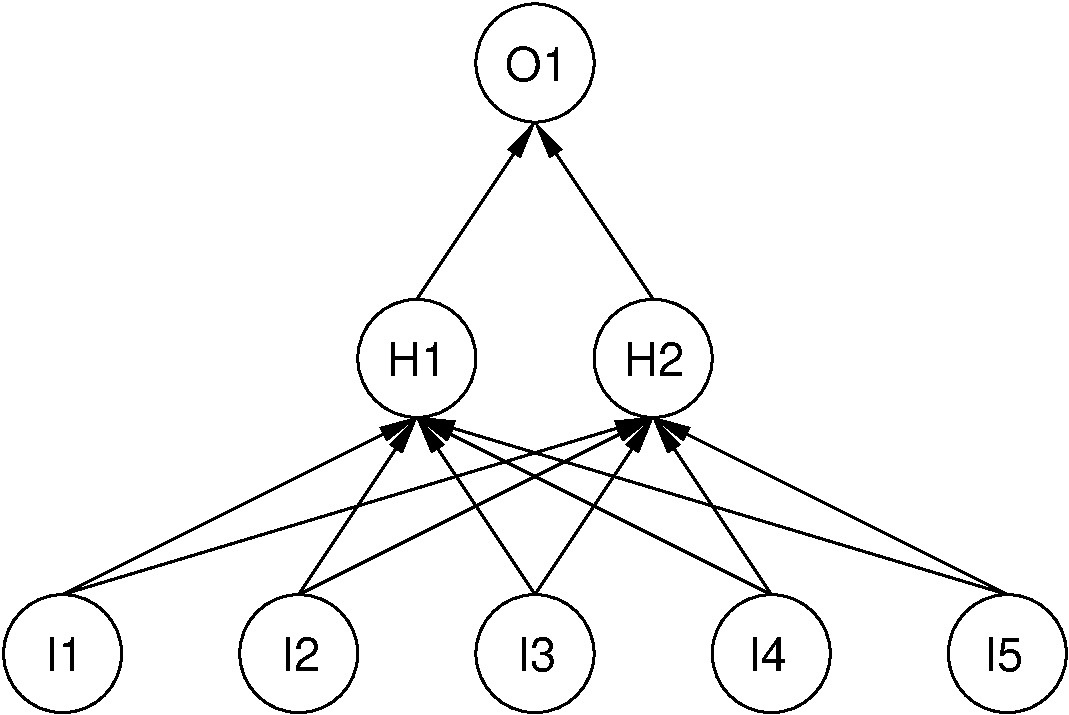
\includegraphics[width=45mm]{figure.pdf}
\caption{This is to show how to include graphics. Always put a reference in the caption where the graph comes from (this one is from the COMP3330 lectures).}
\label{fig:nn1}
\end{center}
\end{figure}

\subsection{Results}
\begin{table}[h!]
    \begin{center}
        \leavevmode
        \begin{tabular}{|cll|l|}\hline
            QR Code & Total number of scans & Number of scans per day\\[0.1cm]\hline
            qr1 & 100 & 1\\\hline
        \end{tabular}
    \end{center}
    \caption{QR Codes}
    \label{table:qrcodes}
\end{table}

\begin{table}[h!]
    \begin{center}
    \leavevmode 
    \small
    \begin{tabular}{|cll|l|}\hline
        %
        QR Code & Total number of scans & Number of scans per day\\[0.1cm]\hline
        %
        NFC1 & 100 & 1\\\hline
    \end{tabular}
    \end{center}
    \caption{NFC Chips}
    \label{table:nfcchips}
\end{table}

\begin{table}[h!]
    \begin{center}
    \leavevmode
    \begin{tabular}{|cll|l|}\hline
        Project & Total Interactions & Interactions per day\\[0.1cm]\hline
        \\\hline
    \end{tabular}
    \end{center}
    \caption{City Evolutions Projects}
    \label{table:cityEvolutionsProjects}
\end{table}

add a graph in of interations over days
\subsection{Just an example table}
We include a table to show how it can be done (see Table~\ref{table:ListOfVelocities}).
%
\begin{table}[h!]
\begin{center}
\leavevmode
%\begin{boxit}
\small %\sf
\begin{tabular}{|cll|l|}\hline
%3
%Speed               & &  & \\3
%
Speed (${mm}/{sec}$) & Methods & Robot & Team, References, Description\\[0.1cm]\hline
%
170& learned & & Sony, \citep{HornbyEtAl1999}??\\%\hline
%
230& hand-tuned & {\sc ers}-210(a) & German Team  \\%\hline
%
245& hand-tuned & {\sc ers}-210(a) &Austin  \\%\hline
%
???& hand-tuned & {\sc ers}-210(a) &NUbots  \\%\hline
%
254& hand-tuned & {\sc ers}-210(a) &UNSW, P-walk of \citep{HengstEtAl2001}\\%\hline
%
270& learned & {\sc ers}-210(a) &UNSW/NICTA, \citep{KimUther2003}\\%\hline
%
295& learned & {\sc ers}-210(a) &NUbots,
\citep{QuinlanChalupMiddletonACRA2003}\\%\hline
%
291& learned & {\sc ers}-210(a) &Austin, \citep{KohlStone2004}\\\hline
%
\end{tabular}
\end{center}
\caption{History of speed improvements for the Sony {\sc aibo}
robot.} \label{table:ListOfVelocities}
\end{table}
%
\section{Discussion}
%
Give an extended and detailed discussion of your study. Explain what we can learn from your study.
%
\section{Glossary}

\section{Conclusion}
%
A brief final summary of the main achievements and outcomes. Possibly some suggestions for future work that can follow on from your project.%
%
\subsection*{Acknowledgements}
The author is grateful to ....
%
\vskip 0.2in
%\newpage
\bibliographystyle{apalike}
\bibliography{./literature.bib}

\end{document}
